\documentclass[sigconf,authorversion,nonacm]{acmart}

\settopmatter{printacmref=false}
\usepackage{xcolor}
\usepackage{graphicx}


%%
%% \BibTeX command to typeset BibTeX logo in the docs
\AtBeginDocument{%
  \providecommand\BibTeX{{%
    Bib\TeX}}}

\begin{document}

\title{CSCI-582 Project Report: "Inference Performance Study on Oak-D Camera"}

\author{Cameron Legg}
\affiliation{%
 \institution{Colorado School of Mines}
 \city{Golden}
 \state{CO}
 \country{USA}
 }

\author{Ben Hempelmann}
\affiliation{%
 \institution{Colorado School of Mines}
 \city{Golden}
 \state{CO}
 \country{USA}
}

\maketitle

\section{Introduction - Cameron}
In this project, we did a study with the Oak-D camera, operating on the Nvidia Orin NX. We vary parameters such as the number of shaves (cores), inference threads, and video size while benchmarking FPS and power consumption. We also run the same benchmark on the CPU and GPU of the Orin NX for extra comparison. Lastly, we discuss what we believe is the optimal number of shaves and inference threads for our model on the Oak-D camera. We run the benchmarks while inferencing human falls with a YOLO model on a 5 minute video.

\section{Targeted domain {\small [2 pts]} - Ben}
Explain the application or the domain you have presented on and experimented with. 

\section{Motivation: The need for acceleration {\small {[2 pts]}} - Cameron}

Detecting human falls may require edge devices to be placed around in many different places. These places could have power restrictions or size restrictions. It is not very practical to place a computer, running a full size graphics card everywhere a camera is needed. In this case, an accelerator is perfect because inferencing can be done rather quickly with a device that is smaller and consumes low power. This is due to the accelerator being designed for that specific application.

\section{Related work {\small {[8 pts]}} - Cameron + Ben}
Starting with the short summary of the paper you presented, explain how other work tackled the acceleration problem for the targeted domain. For the paper you presented, state the key idea(s), solution(s) and contribution(s) of the paper(s) and briefly talk about the technical details of their approach.

You don't need to read additional papers, however, in your summary above, please cite at least 3 other related works that you learned about while you are reading the paper you presented. 

\subsection{Current Limitations - Ben}
Briefly talk about weaknesses of current approaches, if available. 

\section{Project Description  {\small {[2 pts]}} - Cameron}

\subsection{Benchmark}
Our benchmark ran the YOLO model inferencing of the 5 minute video consisting of human falls on the CPU, GPU, and Oak-D camera's accelerator. During the inferencing process, the benchmarking Python script records the average power consumption and FPS over the previous 300 frames. We ran the benchmark many times, altering the number of shaves (cores) and inference threads to be used on the camera's hardware.

\subsection{Accelerated Kernels}
Inferencing with a YOLO model is a highy parallelizable task. This is because many kernels of the inferencing process are parallelizable. For example, a kernel that is can be accelerated is the convolution process. Other kernals, such as activation functions can also be parallelized, making this application perfect for parallelization and acceleration.

\subsection{Targeted Platforms}
We ran the YOLO inferencing benchmark on the following platforms:
\begin{itemize}
    \item \textbf{Nvidia Orin NX GPU} \\ 1024 CUDA Cores
    \item \textbf{Nvidia Orin NX CPU} \\ Arm Cortex A78AE 8-core CPU
    \item \textbf{Oak-D Camera} \\ This camera consists of a system on a chip architecture, running the Intel Movidius Myriad X Vision Processing unit. This accelerator has 2 Leon CPU cores. It also has 16 SHAVE cores - SHAVE cores is company's terminology for vector processing units. This device also has a max power consumption of 4.5W. Lastly, the device has 2 neural compute engines built into the chip.
\end{itemize}

\subsection{Challenges - Ben}
What are the challenges you have faced while using this interface and how you tackled them?
Maybe talk about how we origionally started with the raspberry pi, but couldn't due to need to measure power consumption. Talk about the conversion process. Think of other challenges.

\section{Experiment Setup  {\small {[2 pts]}}}

\subsection{Methodology - Cameron}  

\begin{itemize}
    \item \textbf{Training YOLO} \\ Training the YOLO model was the first step of the process. We found an already-labeled human fall dataset on Kaggle which consisted of 374 images for training and 111 for validation. Each of these images were labeled with Walking, Sitting, and Fall Detected. Essentially, if someone is seen laying down, Fall Detected is triggered. We then used this dataset to train a YOLO v11 model using the T4 GPU in Google Colab.
    \item \textbf{Converting the YOLO PyTorch File} \\ To run the YOLO model on the Oak-D camera, we needed to convert the PyTorch weights file to OpenVino format. The most reliable way to do this conversion was by using the online tool at https://tools.luxonis.com/. This site allows you to upload the PyTorch model and select the number of SHAVEs it should be compiled for. Afterwards, you can download the correctly formatted files and run them directly on the Oak-D camera. 
    \item \textbf{Runtime Framework / Programming Interfaces} \\ - To run the inferencing on the Oak-D camera, we used the Depth AI Python Library, which is a library designed for running inferencing on the Intel Myriad Vector Processor. This library is capable of running the YOLO model after it has been converted to OpenVino format. \\ - To run the inferencing on the CPU and GPU, we used the Ultralytics Python library, which utilizes CUDA when inferencing is done on the Nvidia GPU and OpenMP when inferencing is done on the CPU.
    \item \textbf{Benchmark} \\ The benchmark was written using Python. The script changes the number of SHAVES, and inference threads used while inferencing with YOLO on a 5-minute video. We collected benchmarks for SHAVE numbers 1, 2, 4, 8, 10, 12, 14, and 16 while altering the inference thread numbers 1, 2, 3. We also ran the benchmark on the CPU and GPU. This means that we ran 26 different benchmarks, collecting the average power consumption and frame rate every 300 frames for each benchmark. The benchmark saved these datapoints out to CSV files for each hardware device or shave + thread combination. Because of the way we collected the data (averages every 300 frames), every CSV had the same number of data points, allowing for easier future comparison.
\end{itemize}

\subsection{Metrics measured and Comparisons made - Ben}
What are the metrics (e.g. time, power, energy, etc.) being measured? What is being compared (e.g., applications and/or HW)? Through which methodology? What is your baseline?
CPU GPU Oak-D shaves threads

\section{Results {\small {[9 pts]}}}  
Present your results (with charts) here. For each experiment you did:
\begin{itemize}
    \item Insert a chart/figure/table 
    \item Explain the information that chart/figure/table gives
    \item Interprete results. Refer to more data, if available, to support your interpretation. 
    \item Try to just cover what we talked about in the presentation. Add a little more data on the smaller video file size (352 x 240)
\end{itemize}

There is no min/max limit on the charts. Try to logically group the information if you could. For example, you may include one chart for time measurement, another for power/energy, and another for the breakdown of the performance (data movement overhead, etc.). I expect this to be the most detailed section of your report.

Also, please address the feedback I have given during your project presention.

\begin{itemize}
    \item \textbf{Power consumption VS FPS} \\ For this comparison, we created a scatterplot, comparing the average power consumption over the entire video vs the average FPS over the entire video. 
    \begin{figure}[h] % [h] = here
        \centering
        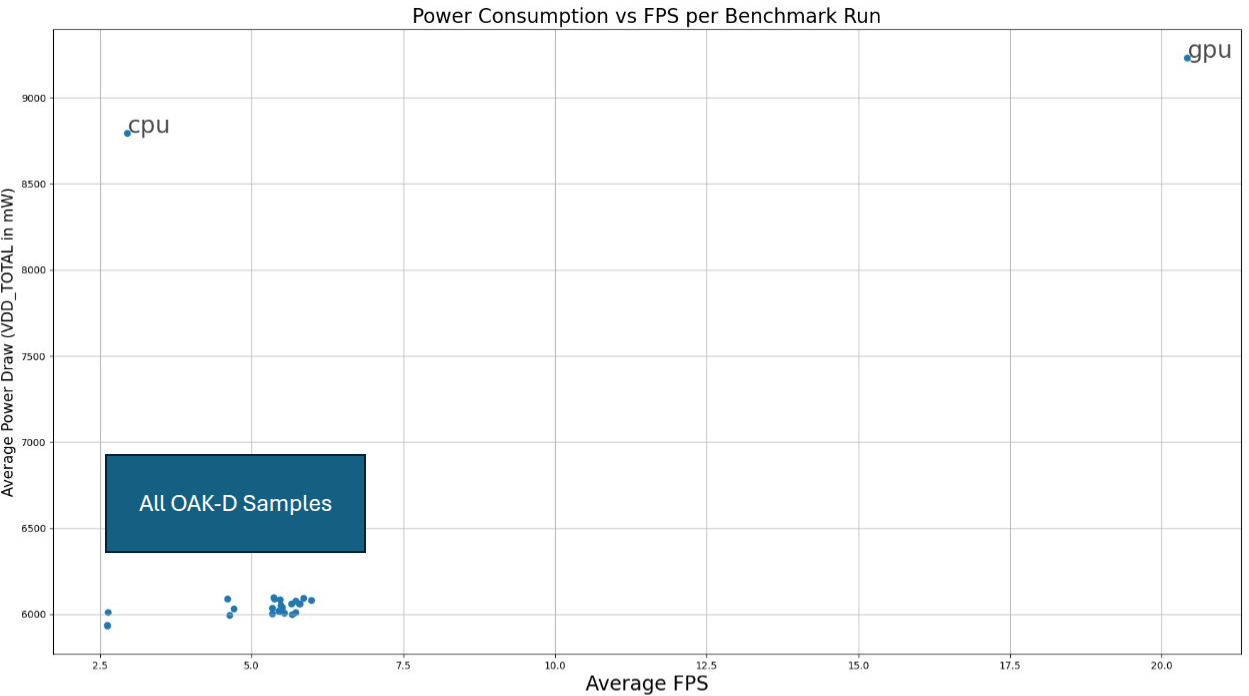
\includegraphics[width=0.5\textwidth]{figures/scatter1.png}
        \caption{Power consumption VS Frame Rate}
        \label{fig:your_label}
    \end{figure}
    \\ In Figure 1, you can see that the GPU consumed lots of power and had a high frame rate. The CPU consumed lots of power, but had a low frame rate. Also, it is visible that the Oak-D samples consumed much less power than the CPU and GPU, and had better frame rates than the CPU.
    \begin{figure}[h] % [h] = here
        \centering
        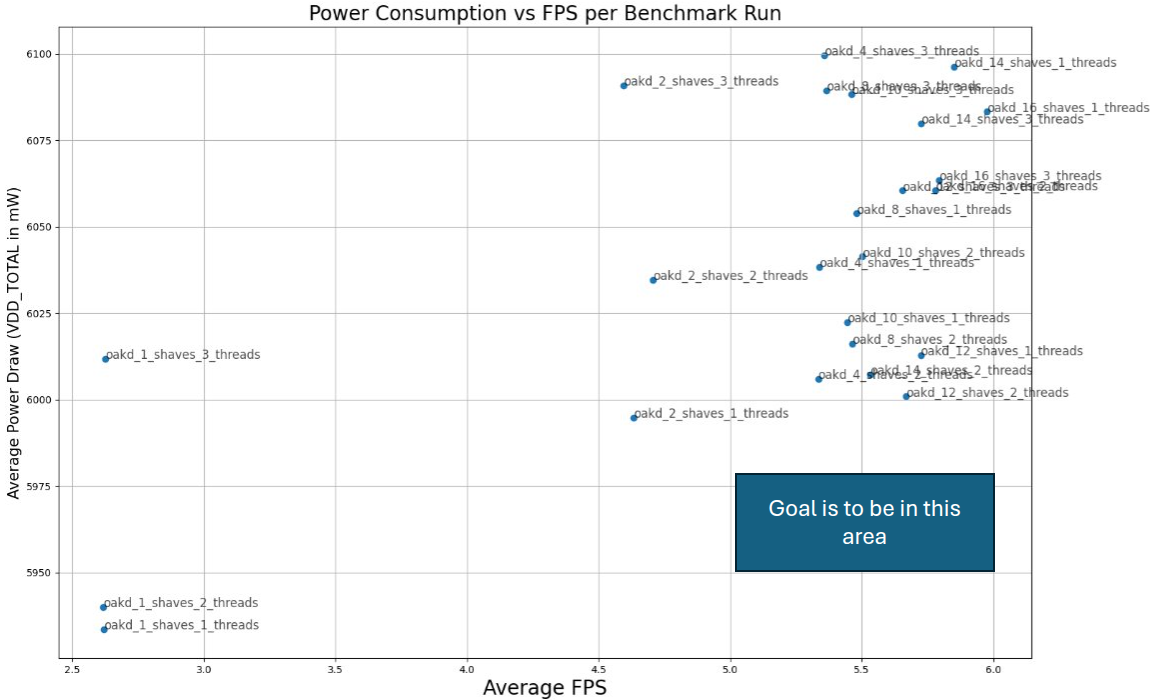
\includegraphics[width=0.5\textwidth]{figures/scatter2.png}
        \caption{Zoomed In - Power consumption VS Frame Rate}
        \label{fig:your_label}
    \end{figure}
    \\ In Figure 2, it is evident that setting the number of SHAVES to 1 resulted in the worst performace, but also lowest power consumption. In general, increasing the number of SHAVES yields a higher performance, but also higher power consumption. For the application of human fall detection on an edge device, an optimal amount of SHAVES and inference threads that yields in high FPS, but low power consumption is ideal. From this scatterplot, we bleieve that running the Oak-D camera with 12 shaves and 2 inference threads results in an optimal power comsumption to FPS ratio.
    
    \item \textbf{Frame vs FPS} \\ For this comparison, we compare the frame number, and the average FPS over the last 300 frames while varying the number of SHAVES, keeping the number of inference threads constant.
    \begin{figure}[h] % [h] = here
        \centering
        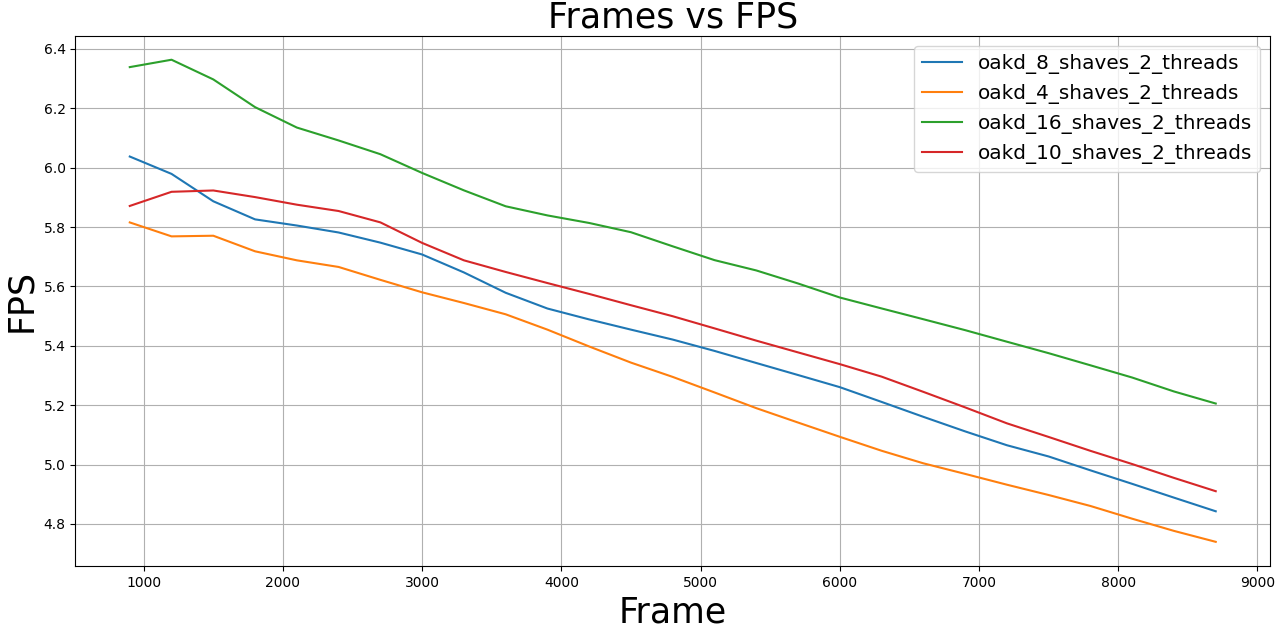
\includegraphics[width=0.5\textwidth]{figures/shavesvfps.png}
        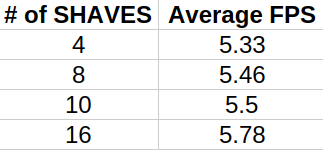
\includegraphics[width=0.2\textwidth]{figures/shavesvfpstable.png}
        \caption{Frame vs FPS}
        \label{fig:your_label}
    \end{figure}
    \\ In Figure 3, the 16 SHAVES model has the highest average FPS at 5.78 FPS, while the 4 SHAVES model has the lowest average FPS at 5.33 FPS. Given this figure, it is evident that increasing the number of SHAVES results in a higher frame rate.
    \item (Ben) Frame vs Power draw -- slide 17
    \item (Ben) power draw for different shaves -- slide 18
    \item (Ben) same shaves, different threads -- slides 19-20
    \item \textbf{Changing Input Video Resolution} \\
    The original 5 minute video we ran for all of the previous benchmarks was 720x480 resolution. Before performing this experiment, we had assumed that decreasing the input video resolution would increase performance, however, we came to the conclusion that it does not. We downsized the same video to 352x240 and ran the same benchmark with that, but the frame rate and power consumption was extremely similar to the previous benchmarks. For example, the Oak-D benchmark with 10 shaves and 2 threads with the smaller video size had an average FPS of 5.81, while the same model on the large video resolution had an FPS of 5.5. This difference is too insignificant to conclude that FPS actually increased.\\ After looking into this issue, we learned that the YOLO models actually scale the resolution up / down to the training photo size before doing inferencing, which was we trained on 640p.
\end{itemize}

\section{Link to Source and other resources {\small {[3 pts]}} - Cameron} 

\begin{itemize}
    \item \textbf{Benchmark Source (made by us) and Results} - \href{https://github.com/cameron-legg/BenchmarkingYOLOOakD}{https://github.com/cameron-legg/BenchmarkingYOLOOakD}
    \item \textbf{Final Presentation} - \href{https://github.com/cameron-legg/BenchmarkingYOLOOakD/blob/main/FinalPresentaiton.pdf}{https://github.com/cameron-legg/BenchmarkingYOLOOakD/blob/main/FinalPresentaiton.pdf}
    \item \textbf{Fall Detection Dataset} - \href{https://www.kaggle.com/datasets/uttejkumarkandagatla/fall-detection-dataset?resource=download}{https://www.kaggle.com/datasets/uttejkumarkandagatla/fall-detection-dataset?resource=download}
    \item \textbf{PyTorch to OpenVino Conversion} - \href{https://tools.luxonis.com/}{https://tools.luxonis.com/}
    \item \textbf{Oak-D Setup} - \href{https://docs.luxonis.com/software/depthai/manual-install/}{https://docs.luxonis.com/software/depthai/manual-install/}
    \item \textbf{A Tutorial We Looked At} - \href{https://learnopencv.com/object-detection-on-edge-device/}{https://learnopencv.com/object-detection-on-edge-device/}
\end{itemize}

\section{Project/class Takeaway {\small {[2 pts]}} - Cameron + Ben}  
Write a brief paragraph on what you have learned ``new" regarding performance analysis and overall on ``compute acceleration". Please also include your honest, brief opinion on how this new knowledge could help your future career. Focus only on what you have learned. I will use this information to evaluate and improve the learning objectives of the class.  \\


During this project we learned the importance of acceleration. We learned that using hardware excelerators can cause more efficient runtime, especially in computer vision applications. We learned that using an accelerator can cause lower power consumption and better frame rate in computer vision applications. Using an accelerator in highly parallelizable applicaitons such as this allows for easier implementaiton of the application onto edge devices that may have power restrictions or even size restrictions.


\section{Feedback {\small {[+1 pts (goes to participation)]}} - Cameron + Ben}  
In addition to the anonymous and official class feedback (which I strongly encourage you to do), please include any other feedback and suggestions (format, content, evaluation, project, etc.) to improve the class. \\

We really enjoyed this class, especially the project portion. The project allowed us to experience real hardware with real applicaitons, which was unique about this class.


\bibliographystyle{ACM-Reference-Format}
\bibliography{references}
[1] A. Raza, M. H. Yousaf and S. A. Velastin, "Human Fall Detection using YOLO: A Real-Time and AI-on-the-Edge Perspective," 2022 12th International Conference on Pattern Recognition Systems (ICPRS), Saint-Etienne, France, 2022, pp. 1-6, doi: 10.1109/ICPRS54038.2022.9854070. keywords: {Image edge detection;Pose estimation;Cameras;Transformers;Real-time systems;Fall detection;Older adults;Computer Vision;Fall Detection;YOLO;OAK-D} \\

[2]




\end{document}